\documentclass[12pt]{article}
\usepackage[english]{babel}
\usepackage[pdftex]{graphicx} 
\usepackage{ragged2e}
\usepackage[margin=1in]{geometry}
\usepackage{listings}
\usepackage{color}
\pagenumbering{gobble}
\lstset{language=Python}
\lstset{frame=lines}
\lstset{label={lst:code_direct}}
\lstset{basicstyle=\footnotesize}
\pagenumbering{roman}
\begin{document}
	\begin{titlepage}
		\centering
		\textsc{\huge \textbf{Minor Project}}\\[1.5cm]
		\textsc{\Large \textbf{Live Audio Gender Recognition using Machine Learning}}\\[0.5cm]
		\textnormal{\\Submitted in partial fulfillment of the requirments for the award of}
		\textnormal{\textbf{\\Degree of Bachelor of Technology}}
		\textnormal{\textbf{\\(Batch: 2014 - 2018)}}
		\textnormal{\\}
		\textnormal{\\By:}
		\textnormal{\\\textbf{Arpit Gogia}}
		\textnormal{\\\textbf{2K14/MC/15}}
		\textnormal{\\}
		\textnormal{\\}
		\textnormal{\\}
		\textnormal{Under the supervision of}
		\textnormal{\\\textbf{Dr. C.P. Singh}}
		\textnormal{\\\textbf{(Assistant Professor)}}
		\textnormal{\\\textbf{(Department of Applied Mathematics)}}
		\textnormal{\\}
		\textnormal{\\}
		\textnormal{\\}
		\textnormal{\\}
		\textnormal{\\}
		
\includegraphics{logo}
		\textnormal{\\}
		\textnormal{\\}
		\textnormal{\\}
		\textnormal{\\\textbf{Delhi Technological University}}
		\textnormal{\\\textbf{Shahbad, Daulatpur, Bawana, Delhi - 110042}}
		\pagebreak
	\end{titlepage}
	\begin{center}
		\textsc{\large \textbf{Declaration}}\\[1.5cm]
	\end{center}
	\textnormal{I hereby certify that the work which is presented in the Minor Project entitled “Live Audio based Gender Recognition using Machine Learning” in fulfillment of the requirement for the award of the Degree of Bachelor of Technology is an authentic record of my own, carried out during a period from January 2017 to May 2017, under the supervision of Dr. C.P. Singh(Assistant Professor, Department of Applied Mathematics). The matter presented in this report has not been submitted by me for the award of any other degree of this or any other Institute/University.}
	\textnormal{\\I acknowledge and understand that plagiarism is wrong. I understand that my research must be accurately referenced. I have followed the rules and conventions concerning referencing, citation and the use of quotations. This assignment is my own work, or my group’s own unique group  assignment. I acknowledge that copying someone else’s assignment, or part of it, is wrong, and that submitting identical work to others constitutes a form of plagiarism. }	
	\textnormal{\\}
	\textnormal{\\}
	\textnormal{\\}
	\textnormal{\\}
	\textnormal{\\}
	\textnormal{\\}
	\begin{flushright}
		\textsc{Arpit Gogia\\}
		\textsc{2K14/MC/15}
	\end{flushright}
	\pagebreak
	\begin{center}
		\textsc{\large \textbf{Supervisor Certificate}}\\[1.5cm]
	\end{center}
	\textnormal{This is to certify that \textbf{ARPIT GOGIA (2K14/MC/015)} a bonafide student of Bachelor of Technology in Mathematics and Computing Engineering of Delhi Technological University, New Delhi of 2014 - 2018 batch has completed his minor project entitled “Live Gender Recognition” under the supervision of \textbf{Dr. C.P. Singh (Assistant Professor, Department of Applied Mathematics)}.}
	\textnormal{It is further certified that the work done in this dissertation is a result of the candidate's own efforts.}
	\textnormal{I wish him all success in his life.\\~\\}
	\begin{flushright}
		Dr. C.P. Singh\\Assistant Professor\\Department of Applied Mathematics\\Delhi Technological University\\Bawana Road, Delhi – 110042\\~\\Date: \underline{\hspace{3cm}}
	\end{flushright}
	\pagebreak
	\begin{center}
		\textsc{\large \textbf{Acknowledgement}}\\[1.5cm]
	\end{center}
	\begin{justify}
		\textnormal{"The successful completion of any task would be incomplete without accomplishing the people who made it all possible and whose constant guidance and encouragement secured us the success".}
	\end{justify}
	\begin{justify}
		\textnormal{I am grateful to Dr. Sangeeta Kansal (HoD, Department of Applied Mathematics) , Delhi Technological University, New Delhi and all other faculty members of our department, for their astute guidance, constant encouragement and sincere support for this project work.}
	\end{justify}
	\begin{justify}
		\textnormal{I owe a debt of gratitude to my guide and mentor, Dr. C.P. Singh (Assistant Professor, Department of Applied Mathematics) for incorporating in me the idea of a creative Minor Project, helping me in undertaking this project and also for being there whenever I needed his assistance.}
	\end{justify}
	\begin{justify}
		\textnormal{I also place on record, my sense of gratitude to one and all, who directly or indirectly have lent their helping hand in this venture. I feel proud and privileged in expressing my deep sense of gratitude to all those who have helped me in presenting this project.}
	\end{justify}
	\begin{justify}
		Last but never the least, I thank my parents for always being with me, in every sense.
	\end{justify}
	\pagebreak
	\begin{center}
		\textsc{\large \textbf{Abstract}}\\[1.5cm]
	\end{center}
	\begin{justify}
		\textnormal{Computers have long been an essential part of our lives. The past few years have seen the rise of computers as extremely powerful computational tools. Machine Learning and Artificial Intelligence domains have flourished in recent times. Computers have gained the power to understand and learn from what we give them to as input. Learning from human generated audio, if achieved to a high accuracy, can be a big advantage of this increased computational power.}
	\end{justify}
	\begin{justify}
		\textnormal{My motive, through this project, is to recognise the gender of subjects using various machine learning techniques on live recorded audio samples. Accomplishing this task would mean a step forward towards improving human-computer interaction, a vital aspect of a robotic system.}
	\end{justify}
	
	\pagebreak
	\tableofcontents
	\pagebreak
	
	\pagebreak
	\pagenumbering{arabic}
	\section{Introduction}
		\subsection{Basics of Machine Learning}
		Machine Learning is a field of computer science that is responsible for giving computers the ability to learn without being explicitly programmed or given instruction to do so. Evolving from pattern recognition and computational learning theory in artificial intelligence, machine learning explores the study of algorithms that can interpret and learn from already available data. Such algorithms can then be used on  large scale to execute data driven decisions. Tom M. Mitchell provided a widely quoted, more formal definition: "A computer program is said to learn from experience E with respect to some class of tasks T and performance measure P if its performance at tasks in T, as measured by P, improves with experience E."
		\subsection{Basics of Deep Learning}
			\begin{justify}
				Deep Learning or Hierarchical Learning is a branch of machine learning based on a set of algorithms that model high level abstractions in data by using a deep graph with multiple processing layers, composed of multiple linear and nonlinear transformations. Deep learning is part of a broader family of machine learning methods based on learning representations of data.
			\end{justify}
			
			\begin{justify}
				An observation or a feature, in machine learning terms, can be represented in many ways like a vector of color values (pixel) of an image, or a vector of frequencies of a music tune. Some features are better at simplify the learning computation.
			\end{justify}
			
			\begin{justify}
				Various deep learning architectures such as deep neural networks, convolutional deep neural networks, deep belief networks and recurrent neural networks have been applied to fields like computer vision, automatic speech recognition, natural language processing, audio recognition and bioinformatics where they have been shown to produce state-of-the-art results on various tasks.
			\end{justify}
			
			\begin{justify}
				Deep Learning algorithms are based on distributed representations of data. The underlying assumption behind distributed assumptions is that observed features originate due to organisation of factors in layers. Varying number of layers and layer sizes provide various levels of abstractions. 
			\end{justify}
			
			\begin{justify}
				Many deep learning algorithms are applied to unsupervised learning tasks. This is an important benefit because unlabeled data are usually more abundant than labeled data. Examples of deep structures that can be trained in an unsupervised manner are neural history compressors and deep belief networks.
			\end{justify}
			\begin{center}
				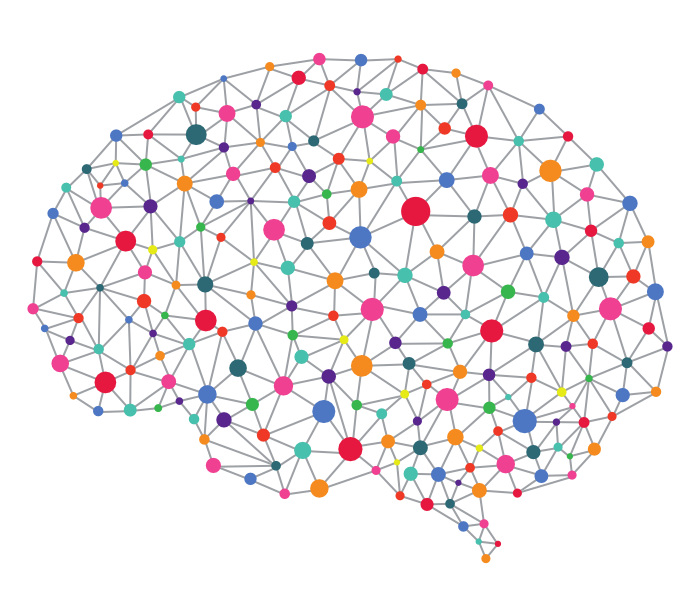
\includegraphics[width=5cm]{dl}
			\end{center}
		\subsection{Audio and Signal Processing}
	\begin{justify}
		Audio signal processing or audio processing is the intentional alteration of audio signals often through an audio effect or effects unit. As audio signals may be electronically represented in either digital or analog format, signal processing may occur in either domain. Analog processors operate directly on the electrical signal, while digital processors operate mathematically on the digital representation of that signal.
	\end{justify}
	\section{Dataset Analysis}
		\subsection{About the dataset}
			\begin{justify}
				This database was created to identify a voice as male or female, based upon acoustic properties of the voice and speech. The dataset consists of 3,168 recorded voice samples, collected from male and female speakers. The voice samples are pre-processed by acoustic analysis in R using the seewave and tuneR packages, with an analyzed frequency range of 0hz-280hz. These voice samples were used for training the various classifiers.
			\end{justify}
		\subsection{Dataset features}
			\begin{justify}
				The dataset has the following acoustic features:
				\begin{enumerate}
					\item \textbf{meanfreq} : \textit{mean frequency (in kHz)}
					\item \textbf{sd} : \textit{standard deviation of frequency}
					\item \textbf{median} : \textit{median frequency (in kHz)}
					\item \textbf{Q25} : \textit{first quartile (in kHz)}
					\item \textbf{Q75} : \textit{third quartile (in kHz)}
					\item \textbf{iqr} : \textit{interquartile range(in kHz)}
					\item \textbf{skew} : \textit{skewness}
					\item \textbf{kurt} : \textit{kurtosis}
					\item \textbf{sp.ent} : \textit{spectral entropy}
					\item \textbf{sfm} : \textit{spectral flatness}
					\item \textbf{mode} : \textit{mode frequency}
					\item \textbf{centroid} : \textit{frequency centroid}
					\item \textbf{peakf} : \textit{peak frequency i.e. frequency with highest energy}
					\item \textbf{meanfun} : \textit{average of fundamental frequency measured across acoustic signal}
					\item \textbf{minfun} : \textit{minimum of fundamental frequency measured across acoustic signal}
					\item \textbf{maxfun} : \textit{maximum of fundamental frequency measured across acoustic signal}
					\item \textbf{meandom} : \textit{average of dominant frequency measured across acoustic signal}
					\item \textbf{mindom} : \textit{minimum of dominant frequency measured across acoustic signal}
					\item \textbf{maxdom} : \textit{maximum of dominant frequency measured across acoustic signal}
					\item \textbf{dfrage} : \textit{range of dominant frequency measured across acoustic signal}
					\item \textbf{modindx} : \textit{modulation index. Calculated as the accumulated absolute difference between adjacent measurements of fundamental frequencies divided by the frequency range}
					\item \textbf{label} : \textit{male or female}
				\end{enumerate}
			\end{justify}
		\subsection{Feature Variation}
		\begin{justify}
			\textnormal{In this section we will observe how the features vary numerically across the category.\\Scatter plots are shown for the original and normalised data. Normalisation is carried out in two steps: \\}
			\begin{center}
				$ x = log(x + 1) $\\
				\textnormal{\\}
				$ x = \frac{x - \bar{x}}{max(x)} $
			\end{center}
			\textbf{meanfreq}\\
				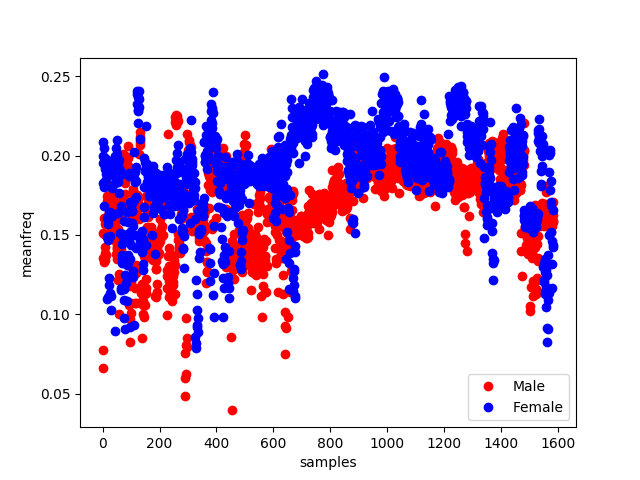
\includegraphics[width=6cm]{../Graphs2/meanfreq}
				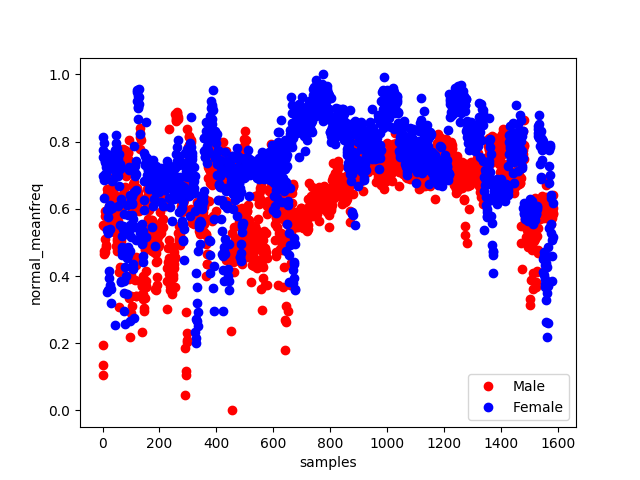
\includegraphics[width=6cm]{../Graphs2/norm_meanfreq}
				
			\textbf{sd}\\
				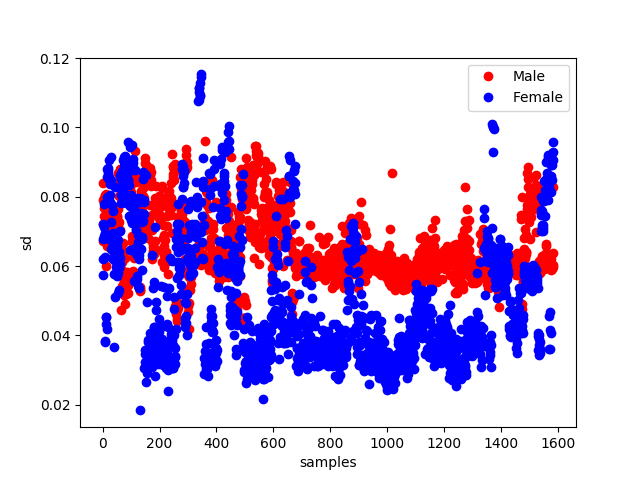
\includegraphics[width=6cm]{../Graphs2/sd}
				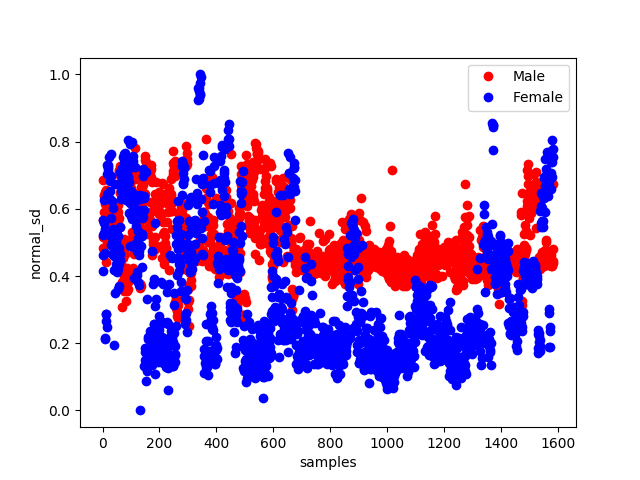
\includegraphics[width=6cm]{../Graphs2/norm_sd}
				
			\textbf{median}\\
				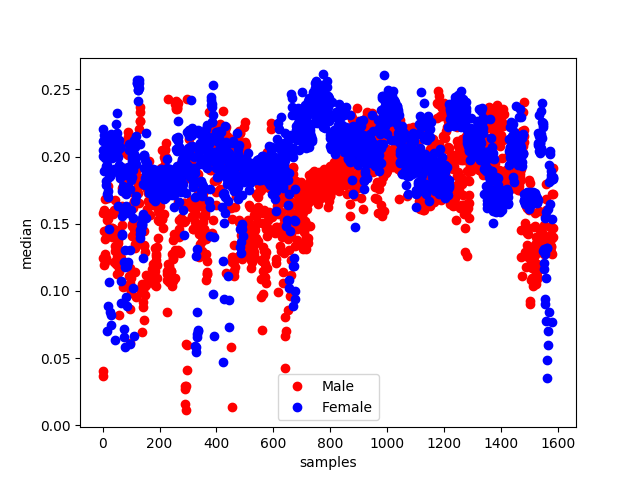
\includegraphics[width=6cm]{../Graphs2/median}
				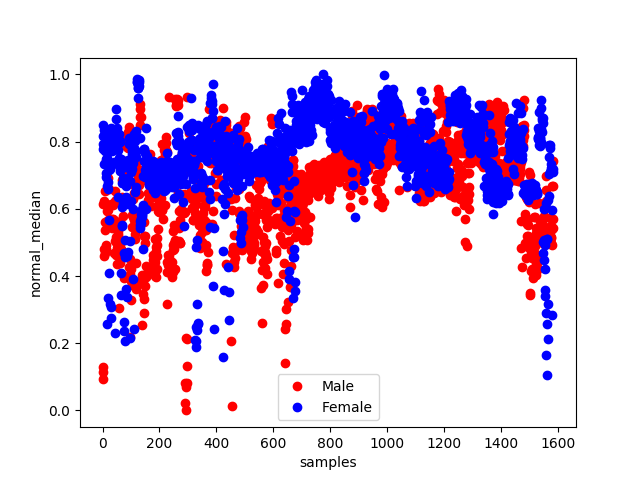
\includegraphics[width=6cm]{../Graphs2/norm_median}
			
			\textbf{Q25}\\
				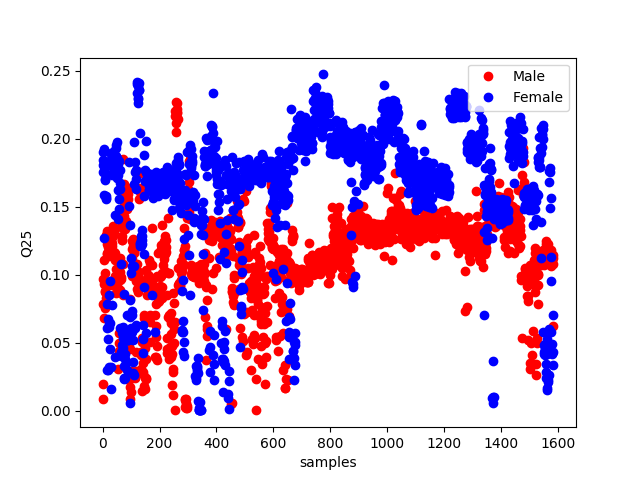
\includegraphics[width=6cm]{../Graphs2/Q25}
				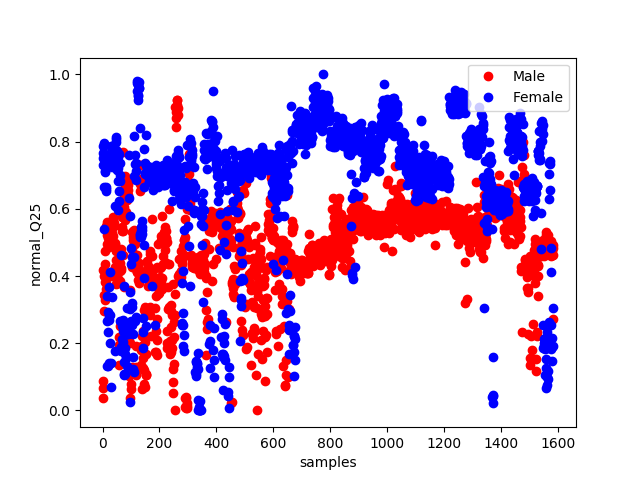
\includegraphics[width=6cm]{../Graphs2/norm_Q25}
				
			\textbf{Q75}\\
				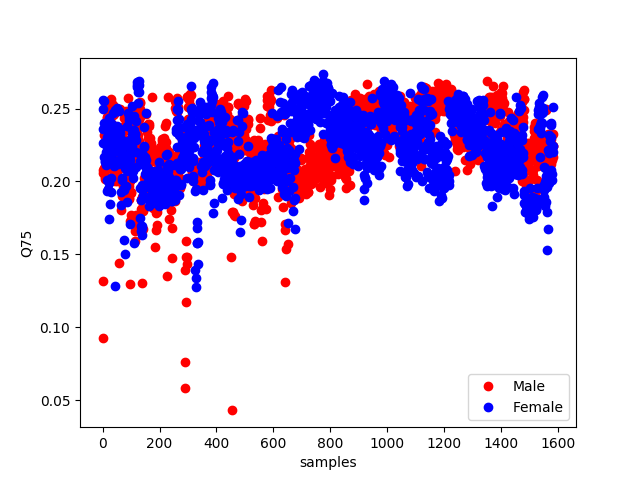
\includegraphics[width=6cm]{../Graphs2/Q75}
				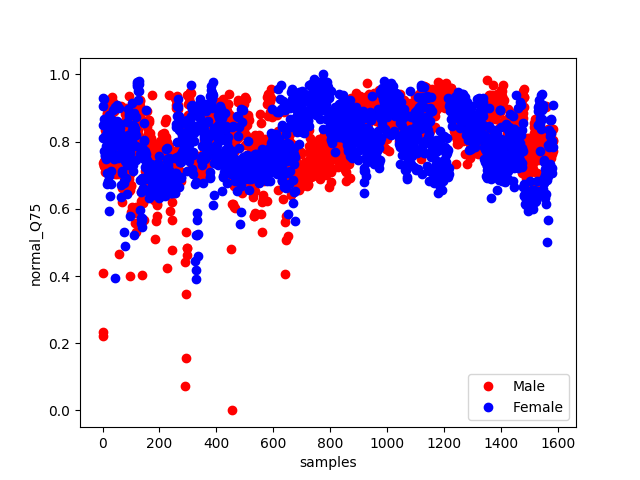
\includegraphics[width=6cm]{../Graphs2/norm_Q75}	
			
			\textbf{IQR}\\
				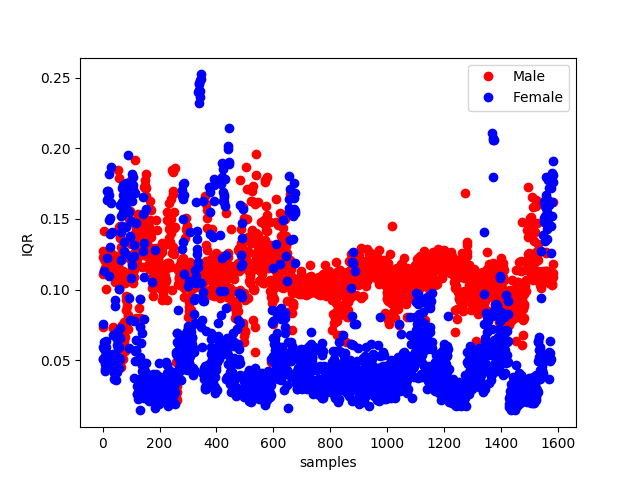
\includegraphics[width=6cm]{../Graphs2/IQR}
				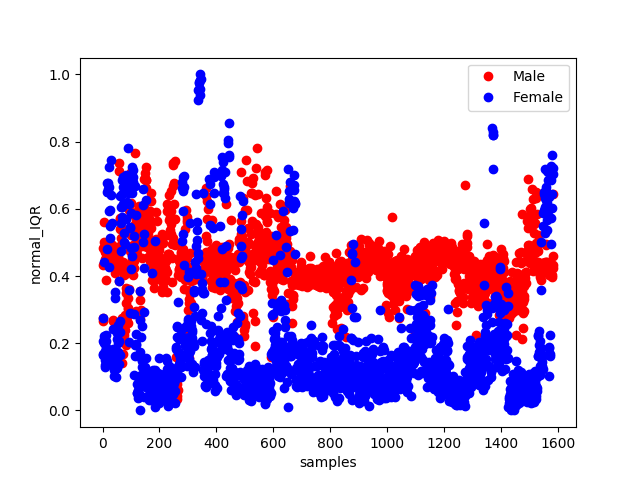
\includegraphics[width=6cm]{../Graphs2/norm_IQR}	
				
			\textbf{skew}\\
				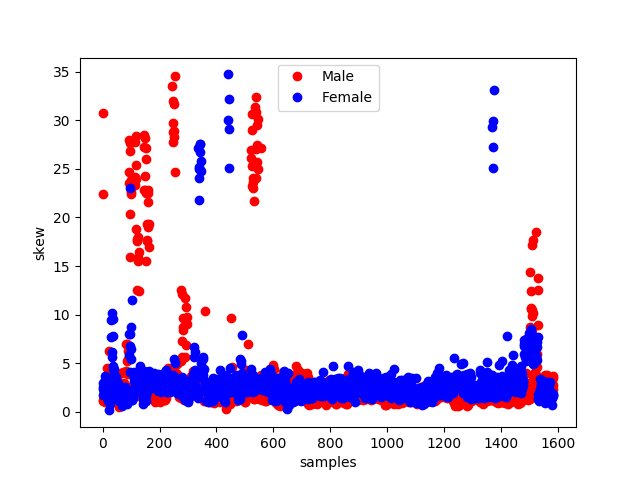
\includegraphics[width=6cm]{../Graphs2/skew}
				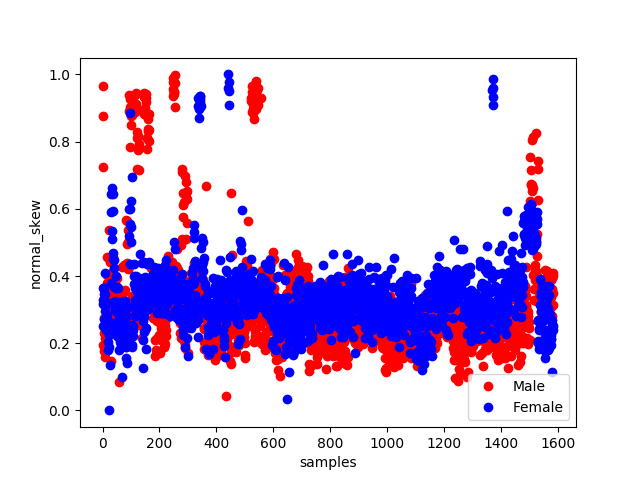
\includegraphics[width=6cm]{../Graphs2/norm_skew}	
				
			\textbf{kurt}\\
				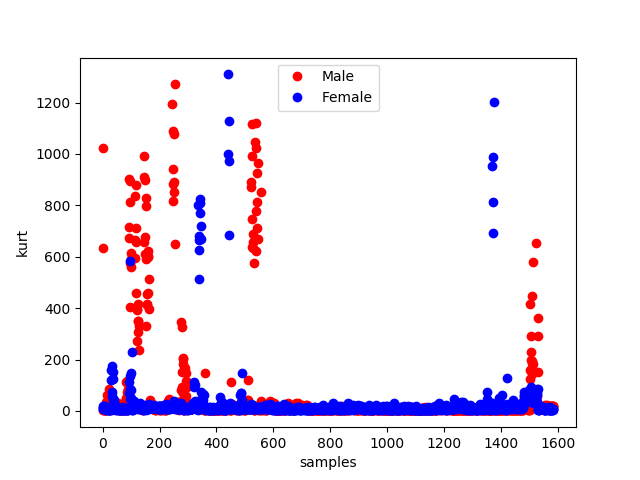
\includegraphics[width=6cm]{../Graphs2/kurt}
				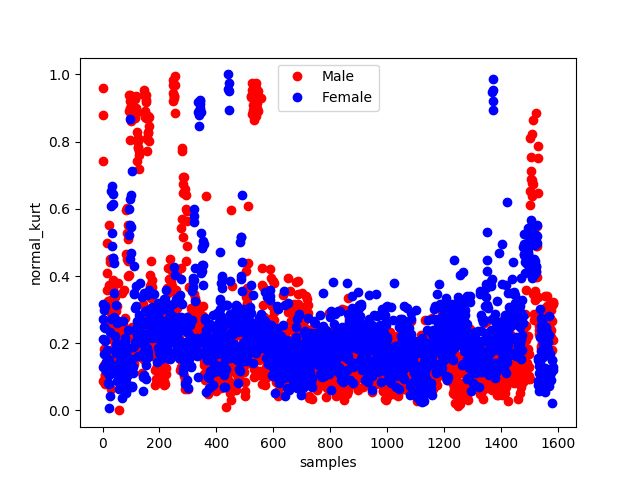
\includegraphics[width=6cm]{../Graphs2/norm_kurt}	
				
			\textbf{sp.ent}\\
				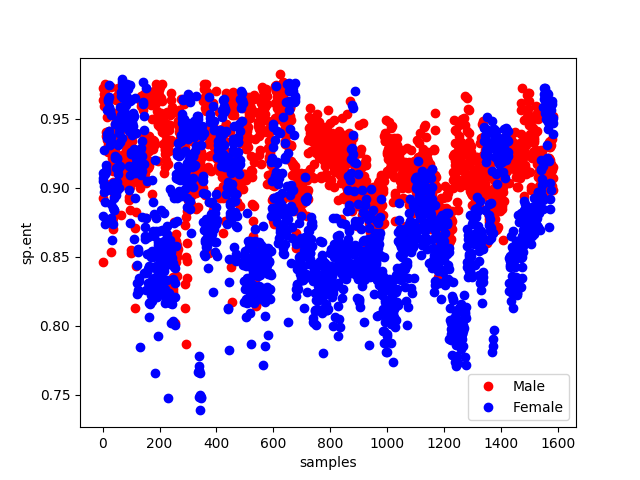
\includegraphics[width=6cm]{../Graphs2/sp_ent.png}
				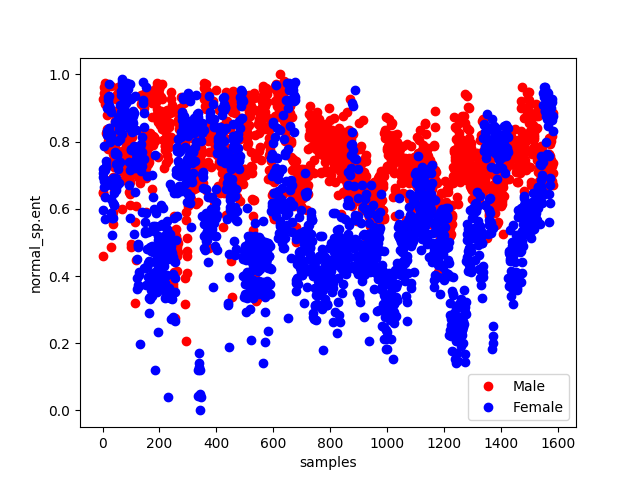
\includegraphics[width=6cm]{../Graphs2/norm_sp_ent.png}	
				
			\textbf{sfm}\\
				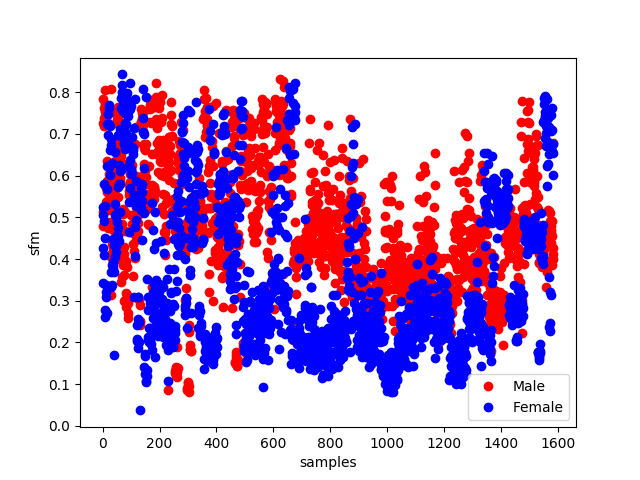
\includegraphics[width=6cm]{../Graphs2/sfm}
				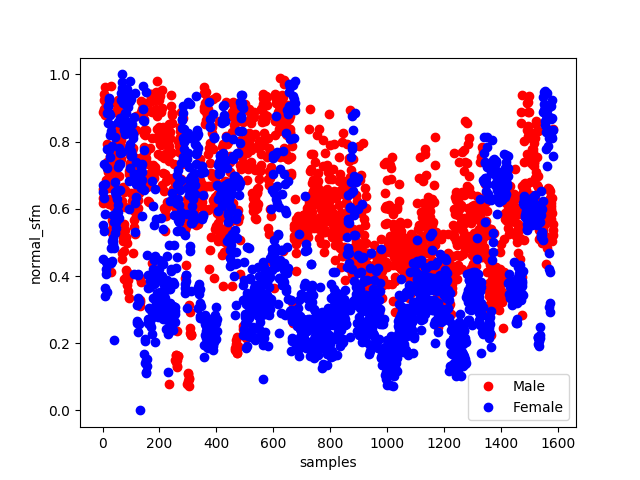
\includegraphics[width=6cm]{../Graphs2/norm_sfm}	
				
			\textbf{mode}\\
				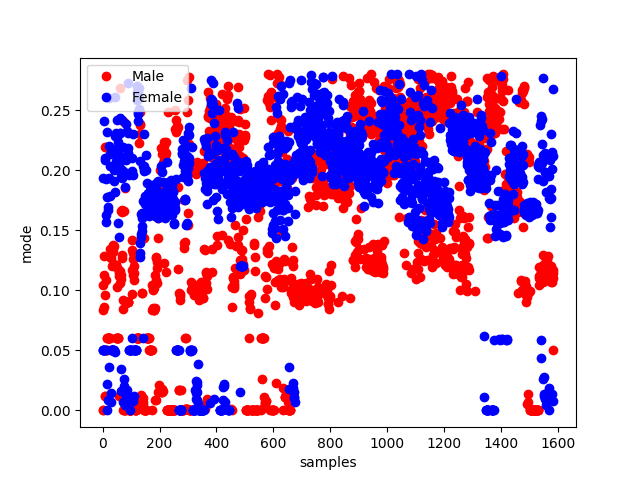
\includegraphics[width=6cm]{../Graphs2/mode}
				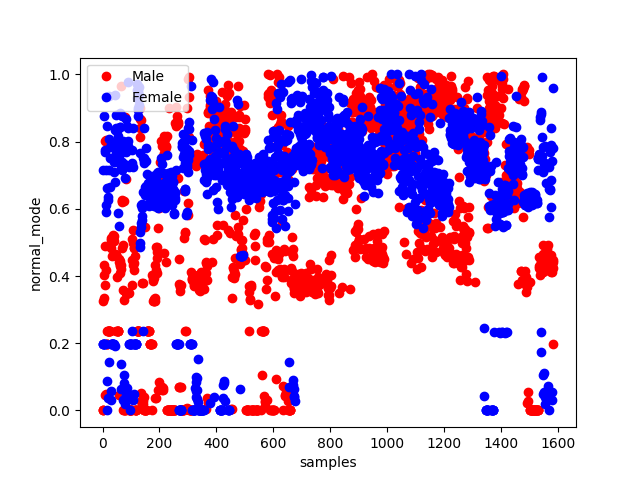
\includegraphics[width=6cm]{../Graphs2/norm_mode}
				
			\textbf{centroid}\\
				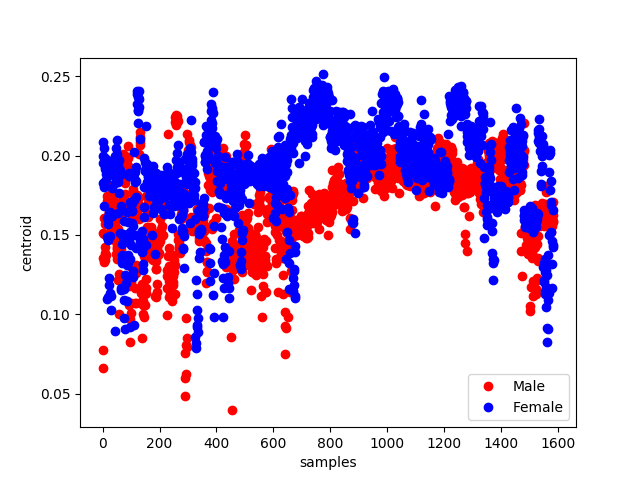
\includegraphics[width=6cm]{../Graphs2/centroid}
				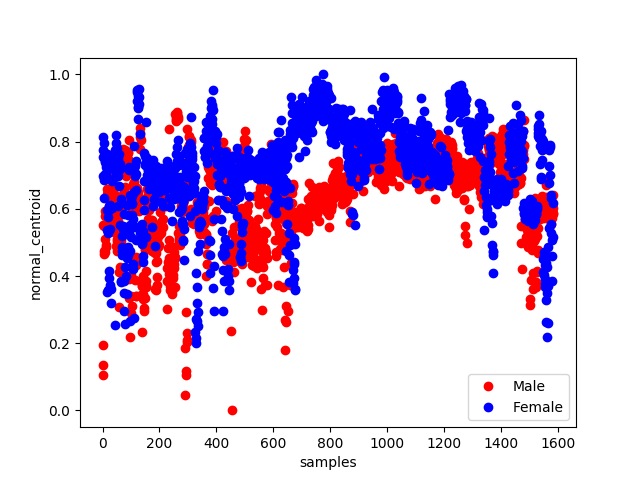
\includegraphics[width=6cm]{../Graphs2/norm_centroid}	
				
			\textbf{meanfun}\\
				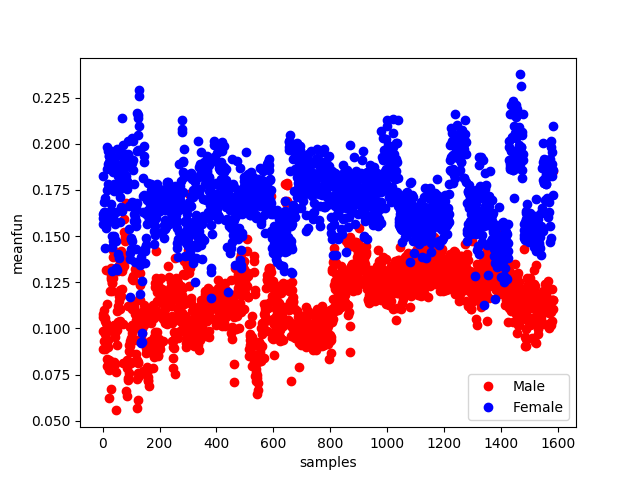
\includegraphics[width=6cm]{../Graphs2/meanfun}
				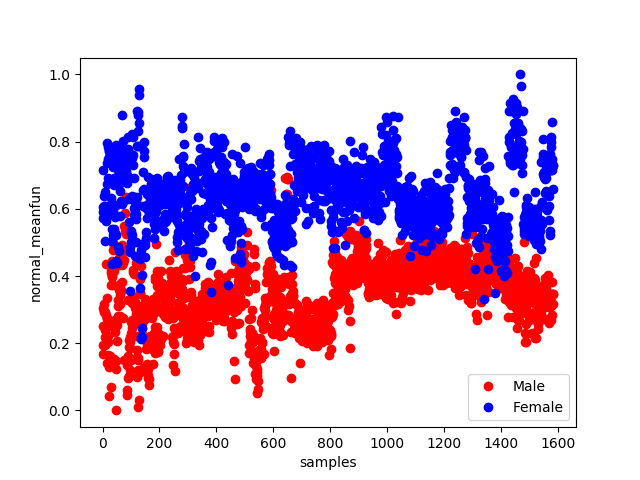
\includegraphics[width=6cm]{../Graphs2/norm_meanfun}	
				
			\textbf{minfun}\\
				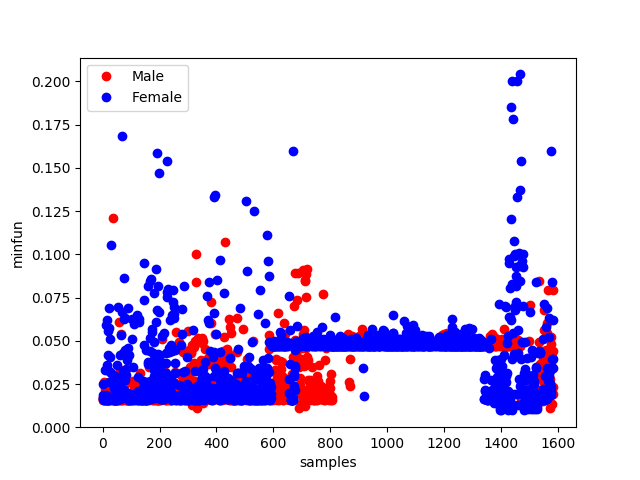
\includegraphics[width=6cm]{../Graphs2/minfun}
				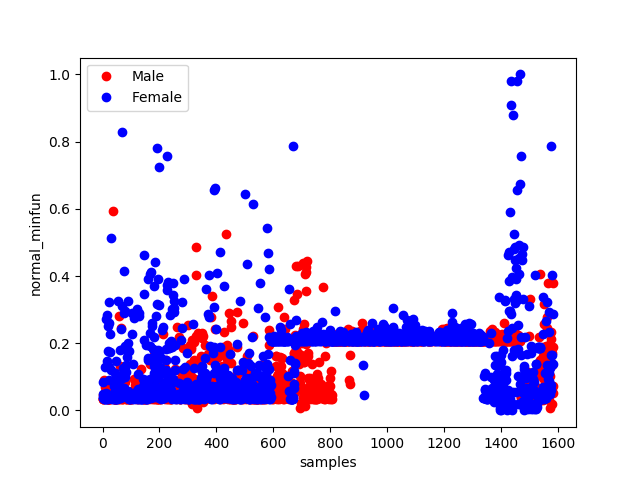
\includegraphics[width=6cm]{../Graphs2/norm_minfun}	
				
			\textbf{meandom}\\
			    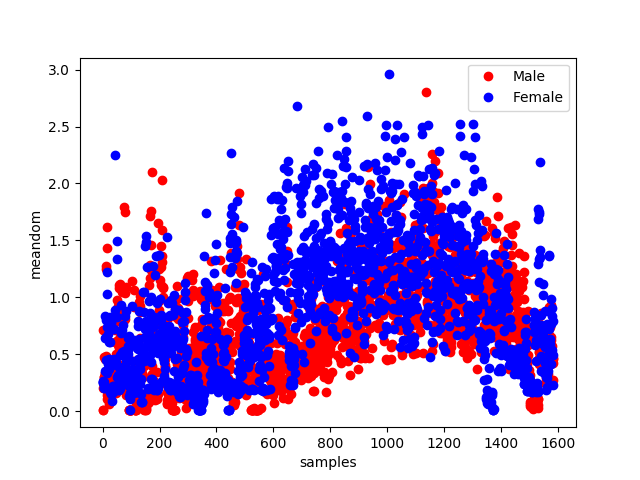
\includegraphics[width=6cm]{../Graphs2/meandom}
				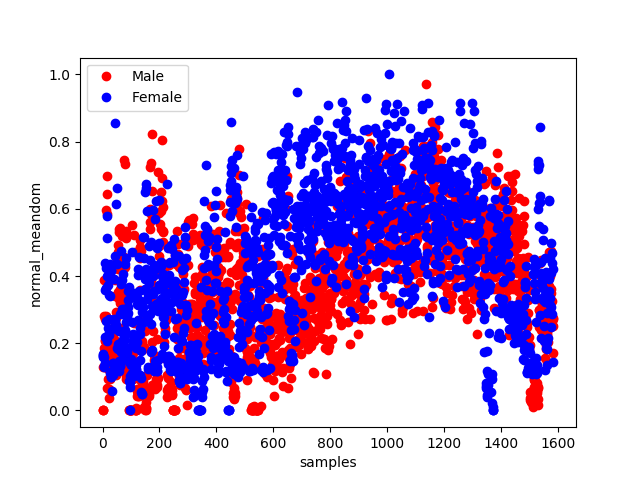
\includegraphics[width=6cm]{../Graphs2/norm_meandom}
				
			\textbf{mindom}\\
				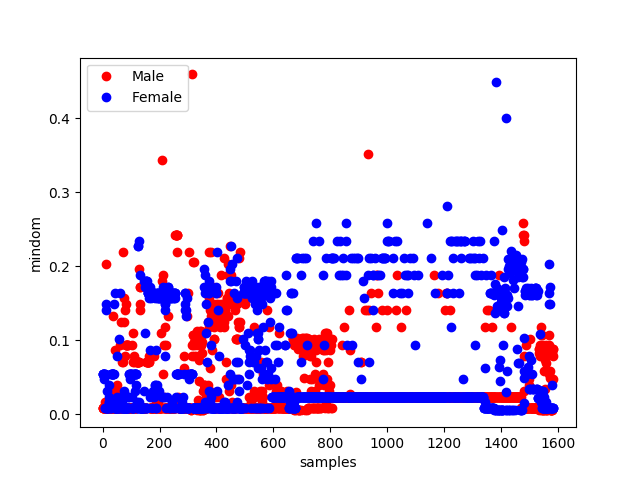
\includegraphics[width=6cm]{../Graphs2/mindom}
				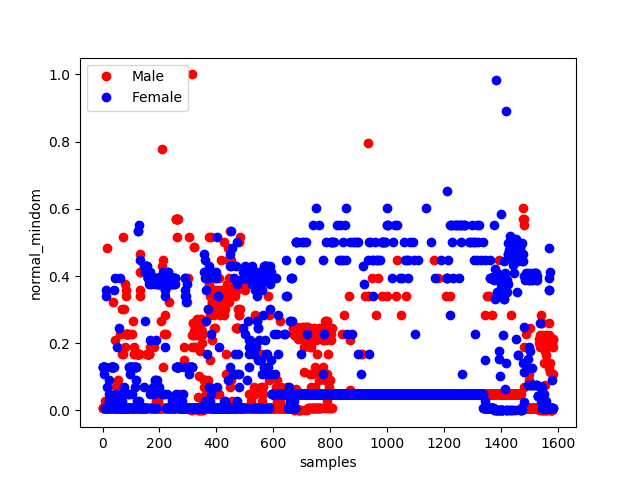
\includegraphics[width=6cm]{../Graphs2/norm_mindom}
				
			\textbf{maxdom}\\
				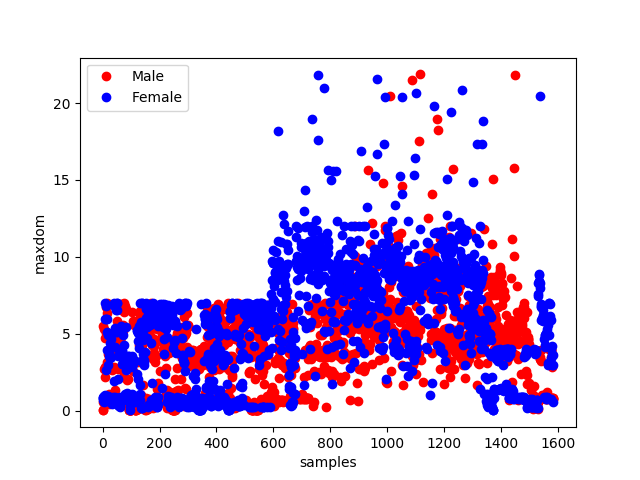
\includegraphics[width=6cm]{../Graphs2/maxdom}
				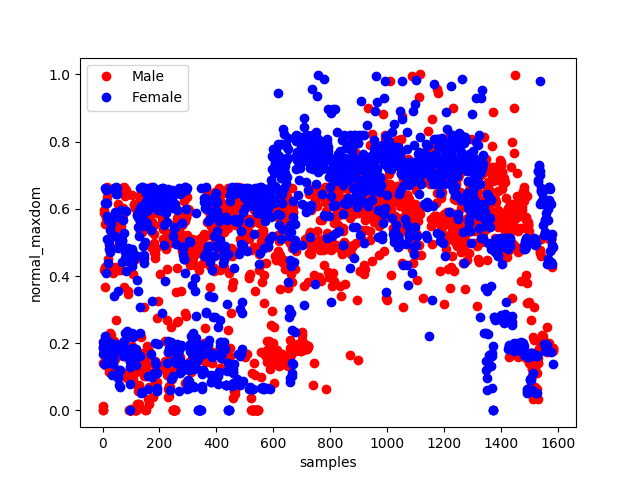
\includegraphics[width=6cm]{../Graphs2/norm_maxdom}	
				
			\textbf{dfrange}\\
				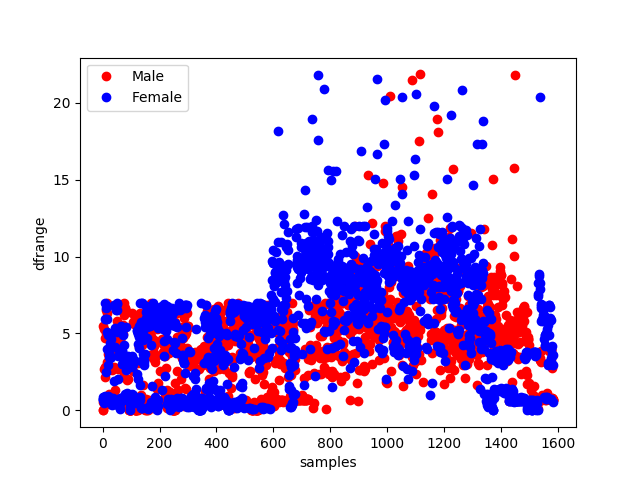
\includegraphics[width=6cm]{../Graphs2/dfrange}
				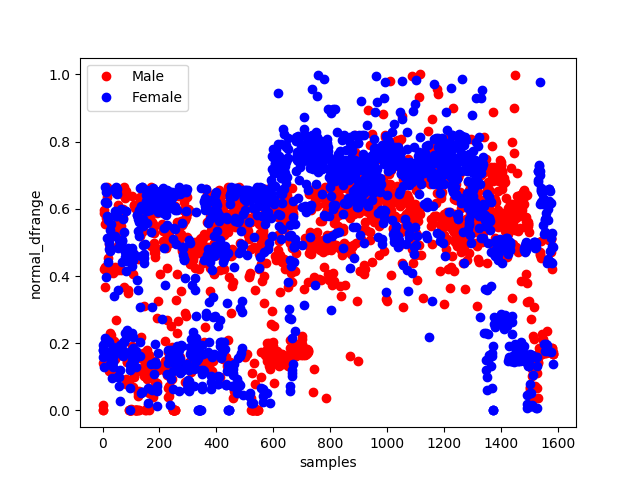
\includegraphics[width=6cm]{../Graphs2/norm_dfrange}	
			
			\textbf{modindx}\\
				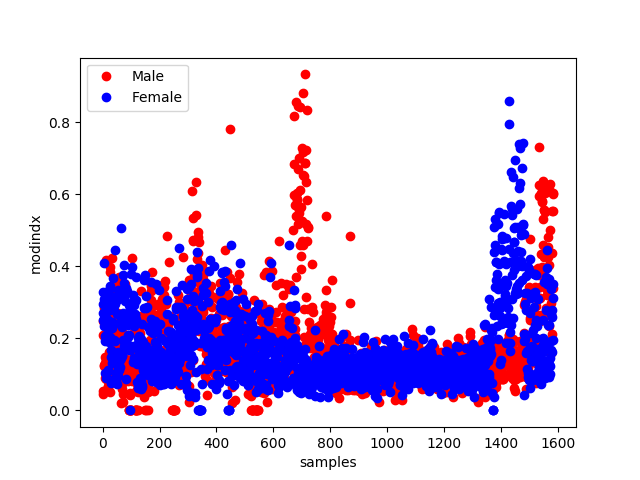
\includegraphics[width=6cm]{../Graphs2/modindx}
				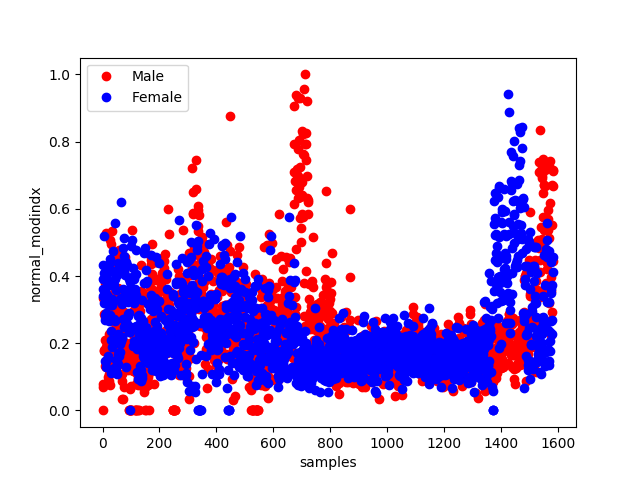
\includegraphics[width=6cm]{../Graphs2/norm_modindx}
				
			\textnormal{\\As we can see from the graphs none of the features individually can visually account for a clearly defined segmentation between the two genders. Mean fundamental frequency comes very close to classifying the samples into the two genders.}
		\end{justify}
	\section{Algorithms and Techniques}
		\subsection{ADA Boost Classifier}
		\begin{justify}
			\textnormal{Boosting is an approach to machine learning based on the idea of creating a highly accurate prediction rule by combining many relatively weak and inaccurate rules. This is done by building a model from the training data, then creating a second model that attempts to correct the errors from the first model. Models are added until the training set is predicted perfectly or a maximum number of models are added. AdaBoost was the first really successful boosting algorithm developed for binary classification. It is the best starting point for understanding boosting.\\\\AdaBoost in general can be used to boost the performance of any machine learning algorithm. It is best used with weak learners, a classifier which is only slightly correlated with the true classification. These are models that achieve accuracy just above random chance on a classification problem.\\\\The most suited and therefore the most common algorithm used with AdaBoost are decision trees with one level. Because these trees are so short and contain only one decision for classification, they are often called decision stumps. Only a binary(two-class) classification problems are supported, so each decision stump make sone decision on one input variable and outputs a +1.0 or -1.0 value for the first or second class value. The misclassification rate is then calculated as follows: \\}
			\begin{center}
				$ error = \frac{correct - N}{N} $ 
			\end{center}
			\textnormal{\\This is then modified to use the weighting of the training instances:}
			\begin{center}
				$ error = sum(w(i) * terror(i)) / sum(w) $
			\end{center}
			which is the weighted sum of the misclassification rate, where w is the weight for training instance i and terror is the prediction error for training instance i which is 1 if misclassified and 0 if correctly classified.\\
			For example if we had 3 training instances with the weights 0.01, 0.5 and 0.2. The predicted values were -1, -1 and -1, and the actual output variables in the instances were -1, 1 and -1, then the terrors would be 0, 1 and 0. The misclassification rate would be calculated as: 
			\begin{center}
				$ error = \frac{0.01 * 0 + 0.5 * 1 + 0.2 * 0}{0.01 + 0.5 + 0.2} $
			\end{center}
			A stage value is calculated for the trained model  which provides a weighting for any predictions that the model makes. The stage value for a trained model is calculated as follows:
			\begin{center}
				$ stage = ln(\frac{1 - error}{error}) $
			\end{center}
			where stage is the stage value used to weight predictions from the model and error is the misclassification error for the model. The effect of the stage weight is that more accurate models have more weight or contribution to the final prediction.\\
			\\The training weights are updated giving more weight to incorrectly predicted instances, and less weight to correctly predicted instances.\\
			\\For example, the weight of one training instance (w) is updated using: 
			\begin{center}
				$ w = w.e^{stage.terror} $
			\end{center}
			where w is the weight for a specific training instance and stage is the misclassification rate for the weak classifier and terror is the error the weak classifier made predicting the output variable for the training instance, evaluated as: 
			\begin{center}
				$ terror = 0 if(y == p), otherwise 1 $
			\end{center}
			where y is the output variable for the training instance and p is the prediction from the weak learner.\\
			\\This has the effect of not changing the weight if the training instance was classified correctly and making the weight slightly larger if the weak learner misclassified the instance.\\
			\\A few things that need to be kept in mind while using an ensemble AdaBoost classifier:
			\begin{itemize}
				\item \textbf{Quality Data: } \textnormal{Because the ensemble method continues to attemp to correct misclassifications in the training data, you need to be careful that the training data is of high-quality.}
				\item \textbf{Outliers: } \textnormal{Outliers will force the ensemble down the rabbit hole of working hard to correct for cases that are unrealistic. These could be removed from the training dataset.}
				\item \textbf{Noisy Data: } \textnormal{Noisy data, specifically noise in the output variable can be problematic. If possible, attempt to isolate and clean these from your training dataset.}
			\end{itemize}
		\end{justify}
		\subsection{Stochastic Gradient Descent Classifier}
		\textnormal{Stochastic Gradient Descent (SGD) is a simple yet very efficient approach to discriminative learning of linear classifiers under convex loss functions such as (linear) Support Vector Machines and Logistic Regression. Even though SGD has been around in the machine learning community for a long time, it has received a considerable amount of attention just recently in the context of large-scale learning.}
		\textnormal{SGD has been successfully applied to large-scale and sparse machine learning problems often encountered in text classification and natural language processing. Given that the data is sparse, the classifiers in this module easily scale to problems with more than $ 10^5 $ training examples and more than $ 10^5 $ features.}
		\textnormal{The SGD classifier gets its importance from its error minimization algorithm known as Stochastic Gradient Descent. Stochastic gradient descent (often shortened in SGD), also known as incremental gradient descent, is a stochastic approximation of the gradient descent optimization method for minimizing an objective function that is written as a sum of differentiable functions. In other words, SGD tries to find minima or maxima by iteration. Gradient Descent is a method to reduce loss/error by moving along the gradient of the loss function. The primary difference between stochastic gradient descent and gradient descent is the fact that in stochastic gradient descent \textbf{only one} sample from the dataset is used to update the weights in each iteration as opposed to multiple samples being used in normal or mini-batch gradient descent. Hence, stochastic gradient descent is faster and converges well before mini-batch gradient descent does.}
		\begin{center}
			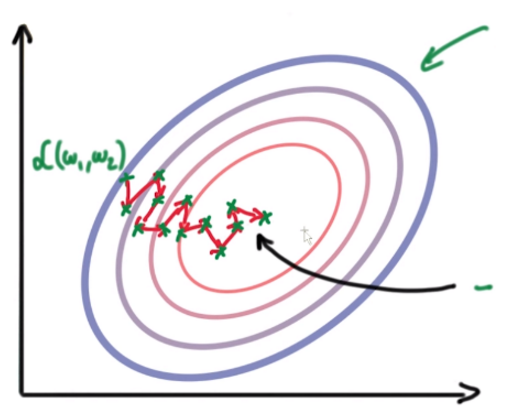
\includegraphics[width=7cm]{sgd}
		\end{center}
		
		\subsection{Decision Tree}
		\textnormal{Decision Trees are a non-paramteric supervised learning method used for oclassisifcation and regression. The goal is to create a model that predicts the value of a target variable by learning simple decision rules inferred from data features.}
		\begin{center}
			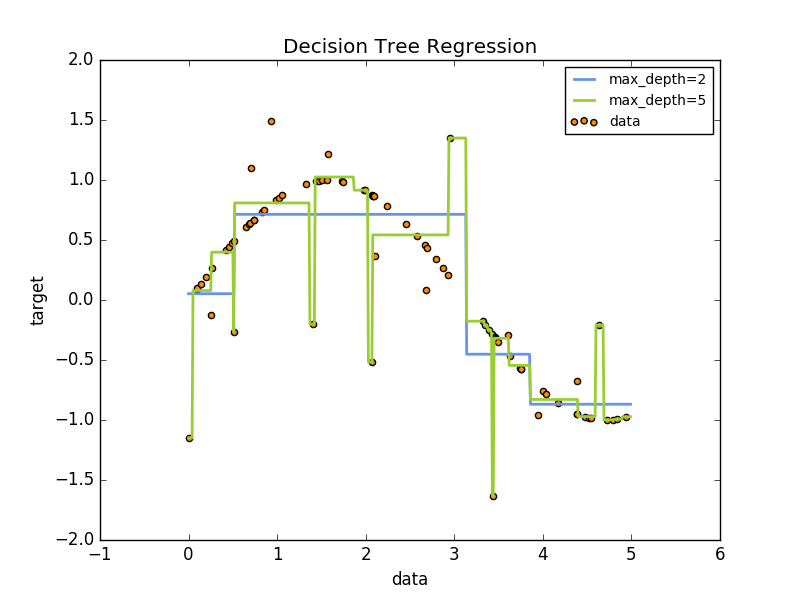
\includegraphics[width=7cm]{dt}
		\end{center}
		Some advantages of decision trees are:
		\begin{itemize}
			\item Simple to understand and to interpret. Trees can be visualised.
			\item Requires little data preparation. Other techniques often require data normalisation, dummy variables need to be created and blank values to be removed. Note however that this module does not support missing values.
			\item The cost of using the tree (i.e., predicting data) is logarithmic in the number of data points used to train the tree.
			Able to handle both numerical and categorical data. Other techniques are usually specialised in analysing datasets that have only one type of variable. See algorithms for more information.
			\item Able to handle multi-output problems.
			Uses a white box model. If a given situation is observable in a model, the explanation for the condition is easily explained by boolean logic. By contrast, in a black box model (e.g., in an artificial neural network), results may be more difficult to interpret.
			\item Possible to validate a model using statistical tests. That makes it possible to account for the reliability of the model.
			\item Performs well even if its assumptions are somewhat violated by the true model from which the data were generated.
			
		\end{itemize}
		The disadvantages of decision trees include:
		\begin{itemize}
			\item Decision-tree learners can create over-complex trees that do not generalise the data well. This is called overfitting. Mechanisms such as pruning (not currently supported), setting the minimum number of samples required at a leaf node or setting the maximum depth of the tree are necessary to avoid this problem.
			\item Decision trees can be unstable because small variations in the data might result in a completely different tree being generated. This problem is mitigated by using decision trees within an ensemble.
			\item The problem of learning an optimal decision tree is known to be NP-complete under several aspects of optimality and even for simple concepts. Consequently, practical decision-tree learning algorithms are based on heuristic algorithms such as the greedy algorithm where locally optimal decisions are made at each node. Such algorithms cannot guarantee to return the globally optimal decision tree. This can be mitigated by training multiple trees in an ensemble learner, where the features and samples are randomly sampled with replacement.
			\item There are concepts that are hard to learn because decision trees do not express them easily, such as XOR, parity or multiplexer problems.
			\item Decision tree learners create biased trees if some classes dominate. It is therefore recommended to balance the dataset prior to fitting with the decision tree.
		\end{itemize}
		\subsection{Random Forest Classifier}
		\begin{justify}
			Random forests or random decision forests[1][2] are an ensemble learning method for classification, regression and other tasks, that operate by constructing a multitude of decision trees at training time and outputting the class that is the mode of the classes (classification) or mean prediction (regression) of the individual trees. Random decision forests correct for decision trees' habit of overfitting to their training set.
			The training algorithm for random forests applies the general technique of bootstrap aggregating, or bagging, to tree learners. Given a training set $ X = x_{1}, ..., x_{n}$  with responses $ Y = y_{1}, ..., y_{n} $ bagging repeatedly (B times) selects a random sample with replacement of the training set and fits trees to these samples. For $ b = 1, ..., B $:
			\begin{itemize}
				\item Sample, with replacement, \textit{B} training examples from X, Y; call these Xb, Yb.
				\item Train a decision or regression tree fb on Xb, Yb.
			\end{itemize}
		After training, predictions for unseen samples x' can be made by averaging the predictions from all the individual regression trees on x':
		\begin{center}
			$ {\displaystyle {\hat {f}}={\frac {1}{B}}\sum _{b=1}^{B}f_{b}(x')} {\displaystyle {\hat {f}}={\frac {1}{B}}\sum _{b=1}^{B}f_{b}(x')} $
		\end{center}
		or by taking the majority vote in the case of decision trees.
		This bootstrapping procedure leads to better model performance because it decreases the variance of the model, without increasing the bias. This means that while the predictions of a single tree are highly sensitive to noise in its training set, the average of many trees is not, as long as the trees are not correlated. Simply training many trees on a single training set would give strongly correlated trees (or even the same tree many times, if the training algorithm is deterministic); bootstrap sampling is a way of de-correlating the trees by showing them different training sets. \\The number of samples/trees, B, is a free parameter. Typically, a few hundred to several thousand trees are used, depending on the size and nature of the training set. An optimal number of trees B can be found using cross-validation, or by observing the out-of-bag error: the mean prediction error on each training sample xᵢ, using only the trees that did not have xᵢ in their bootstrap sample. The training and test error tend to level off after some number of trees have been fit.\\The above procedure describes the original bagging algorithm for trees. Random forests differ in only one way from this general scheme: they use a modified tree learning algorithm that selects, at each candidate split in the learning process, a random subset of the features. This process is sometimes called "feature bagging". The reason for doing this is the correlation of the trees in an ordinary bootstrap sample: if one or a few features are very strong predictors for the response variable (target output), these features will be selected in many of the B trees, causing them to become correlated. An analysis of how bagging and random subspace projection contribute to accuracy gains under different conditions is given by Ho. Typically, for a classification problem with p features, $ \sqrt{p} $ (rounded down) features are used in each split. For regression problems the inventors recommend p/3 (rounded down) with a minimum node size of 5 as the default.
		\end{justify}
		\subsection{Naive Bayes Classifier}
		\begin{justify}
			The Bayesian Classification represents a supervised learning method as well as a statistical method for classification. Assumes an underlying probabilistic model and it allows us to capture uncertainty about the model in a principled way by determining probabilities of the outcomes. It can solve diagnostic and predictive problems. This Classification is named after Thomas Bayes (1702-1761), who proposed the Bayes Theorem. Bayesian classification provides practical learning algorithms and prior knowledge and observed data can be combined. Bayesian Classification provides a useful perspective for understanding and evaluating many learning algorithms. It calculates explicit probabilities for hypothesis and it is robust to noise in input data. \\Naïve Bayes Algorithm is based on the Bayesian theorem It is particularly suited when the dimensionality of the inputs is high. Parameter estimation for naive Bayes models uses the method of maximum likelihood. In spite over-simplified assumptions, it often performs better in many complex real world situations Advantage: Requires a small amount of training data to estimate the parameters.
			\begin{center}
				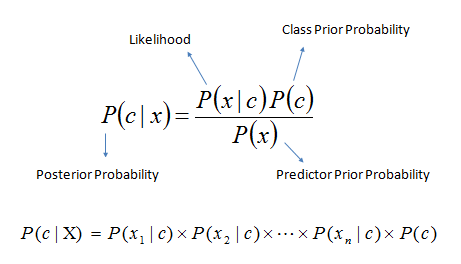
\includegraphics[width=7cm]{nb}
			\end{center}
		\end{justify}
	\section{Languages and Frameworks}
		\subsection{Python}
		\textnormal{Python is a high-level, general purpose, interpreted, dynamic programming language which focuses primarily on increased readability of code. Its syntax is closer to spoken english and allows programmers to use comparatively fewer lines of code, as opposed to the more popular languages like C++ or Java. Python is highly platform independent and interpreters are available for all popular operating systems. Common tools like py2exe or pyInstaller allow python programs to be packaged into operating system level executables allowing execution of the program even without a Python interpreter installed.\\All the code for modeling, training, predicting and analysis has been written in Python 2.7.}
		\subsection{Sounddevice}
		A simple Python module that provides bindings for the PortAudio library. This module helps in recording and playing WAV files. I picked this library because it returns a NumPy array of amplitudes after recording the sound.
		
		\subsection{NumPy}
		NumPy is an extension to the Python programming language, adding support for large, multidimensional arrays and matrices, along with a large library of high-level mathematical functions to operate on these arrays. The ancestor of NumPy, Numeric, was originally created by Jim Hugunin with contributions from several other developers. In 2005, Travis Oliphant created NumPy by incorporating features of the competing Numarray into Numeric, with extensive modifications. NumPy is open source and has many contributors.
		
		\subsection{SciPy}
		SciPy is an open source Python library used for scientific computing and technical computing.
		\\SciPy contains modules for optimization, linear algebra, integration, interpolation, special functions, signal and image processing, ODE solvers and other tasks common in science and engineering.
		SciPy builds on the NumPy array object and is part of the NumPy stack which includes tools like Matplotlib, pandas and SymPy. There is an expanding set of scientific computing libraries that are being added to the NumPy stack every day. This NumPy stack has similar users to other applications such as MATLAB, GNU Octave, and Scilab. The NumPy stack is also sometimes referred to as the SciPy stack.
		
		\subsection{Matplotlib}
		Matplotlib is a plotting library for the Python programming language and its numerical mathematics extension NumPy. It provides an object-oriented API for embedding plots into applications using general-purpose GUI toolkits like wxPython, Qt, or GTK+. There is also a procedural "pylab" interface based on a state machine (like OpenGL), designed to closely resemble that of MATLAB. SciPy makes use of matplotlib. All the graphs for analysis have been plotted using matplotlib.
		
		\subsection{R and RPy2}
		R is an open source programming language and software environment for statistical computing and graphics that is supported by the R Foundation for Statistical Computing. The R language is widely used among statisticians and data miners for developing statistical software and data analysis. Polls, surveys of data miners, and studies of scholarly literature databases show that R's popularity has increased substantially in recent years.\\R is a GNU package. The source code for the R software environment is written primarily in C, Fortran, and R. R is freely available under the GNU General Public License, and pre-compiled binary versions are provided for various operating systems. While R has a command line interface, there are several graphical front-ends available.\\R as a language was not explicitly used in this project, however, the dataset I obtained was built after processing audio files using R packages specializing in signal processing. The specific package used is called \textbf{seewave}. To process the incoming live audio, I have used the python bridge module to R named \textbf{RPy2}. It maps R objects and functions to the python interface for easy use.
		
		\subsection{WAV Audio format}
		Waveform Audio File Format (WAVE, or more commonly known as WAV due to its filename extension) (rarely, Audio for Windows) is a Microsoft and IBM audio file format standard for storing an audio bitstream on PCs. It is an application of the Resource Interchange File Format (RIFF) bitstream format method for storing data in "chunks", and thus is also close to the 8SVX and the AIFF format used on Amiga and Macintosh computers, respectively. It is the main format used on Windows systems for raw and typically uncompressed audio. The usual bitstream encoding is the linear pulse-code modulation (LPCM) format.  The format takes into account some differences of the Intel CPU such as little-endian byte order. The RIFF format acts as a "wrapper" for various audio coding formats. Though a WAV file can contain compressed audio, the most common WAV audio format is uncompressed audio in the linear pulse code modulation (LPCM) format. LPCM is also the standard audio coding format for audio CDs, which store two-channel LPCM audio sampled 44,100 times per second with 16 bits per sample. Since LPCM is uncompressed and retains all of the samples of an audio track, professional users or audio experts may use the WAV format with LPCM audio for maximum audio quality. WAV files can also be edited and manipulated with relative ease using software.
		
	\section{Code and Implementation}
		The main python scripts are \textbf{record.py} and \textbf{prediction.py}.
		\subsection{record.py}
			This script handles audio recording for gender prediction. It also calls the prediction function to predict the gender of the recorded audio.\\
			\lstinputlisting[language=Python, firstline=1, lastline=9]{../record.py}
			In the above code, I import the necessary modules \textbf{rpy2} for getting the features from the recorded audio using R packages; and \textbf{sounddevice} for recording the audio.\\
			\lstinputlisting[firstline=10, lastline=12]{../record.py}
			These three lines of code import the required R packages through rpy2.\\
			\lstinputlisting[firstline=15, lastline=23]{../record.py}
			This function records audio from the user's microphone. The duration of the recorded audio sample is fixed at 3 seconds. The sample rate is also fixed at a standard 44100 kHz.\\
			\lstinputlisting[firstline=26, lastline=62]{../record.py}
			This function is a crucial part of the script. It calls \textbf{get\_audio()} to record the audio and save it in \textbf{test.wav}. The next lines call the required R package functions to calculate all the required features.\\
			\lstinputlisting[firstline=64, lastline=65]{../record.py}
			The prediction object is created and the classifiers are trained. To get the results from the classifiers, the \textbf{predict()} function is called.
		\subsection{prediction.py}
			This script defines the prediction class which is responsible for training the classifiers using the Kaggle dataset.\\
			\lstinputlisting[firstline=24, lastline=97]{../prediction.py}
			This is the constructor of the Prediction object. It trains the classifiers and attaches them to the objects for further use. Before the classification, the features are normalised and reduced to the range \textbf{(0, 1)}.\\
			After doing that, the 6 classifiers are trained on the data. The classifiers can have various hyper parameters that need to be tuned. Grid Search has been used to find the most optimal classifier by trying many permutations of the various settings.\\
			\lstinputlisting[firstline=99, lastline=126]{../prediction.py}
			The pre-trained classifiers are used to predict the gender of the recorded audio. The prediction and audio features are then appended to the csv file to be stored for future training.
	\section{Observations}
	
		\begin{center}
			\begin{tabular}{ | l | c | r }
				\hline
				\textbf{Classifier} & \textbf{Testing Accuracy} \\ \hline
				SGD & 0.961759 \\ \hline
				Decision Tree & 0.9550669 \\ \hline
				AdaBoost & 0.9665391 \\ \hline
				Random Forest & 0.9665391 \\ \hline
				Naive Bayes & 0.97036328 \\ \hline
				Support Vector & 0.9684512 \\ \hline
			\end{tabular}
		\end{center}
	\section{Applications and Future Scope}
		There exist a number of applications which can benefit from automatic facial gender and emotion recognition. Voice emotion and gender recognition provide essential context while answering a question. Being able to recognize voice expressions can assist voice recognition algorithms. Furthermore, body language is an important part of human-human communication. Developing methods for a computer to automatically recognize human expressions, could enhance the quality of human-computer interaction and enable the construction of more natural adaptive interfaces and environments. Recognition of expressions in voice is useful for ’adapting interactive feedback in a tutoring system based on the student’s level of interest, or for monitoring pilots and drivers’ alertness state. Automatic recognition could also be used on video recording of group interactions, to trace and document changes in the expressions of the participants, or to retrieve pieces of a video based upon a particular expression of a subject. Yet another application is found in the development of psychological emotion theories by facilitating the experimental data collection of facial expressions associated with particular emotions. The recognition of gender and emotion in voice would further facilitate Personal Assistants such as Siri and Google Now to interact in a better way with their user keeping in mind, their expressions at that state and using the correct pronouns to identify the user. 
	\pagebreak
	\section{Appendix}
	\begin{center}
		\textbf{\large record.py}
	\end{center}
	\lstinputlisting{../record.py}
	\pagebreak
	\begin{center}
		\textbf{\large prediction.py}
	\end{center}
	\lstinputlisting{../prediction.py}
	\pagebreak
	\begin{center}
		\textbf{\large graphs.py}
	\end{center}
	\lstinputlisting{../graphs.py}
	\pagebreak
	\section{References}
	\begin{enumerate}
		\item Explaining AdaBoost - http://rob.schapire.net/papers/explaining-adaboost.pdf
		\item Boosting and AdaBoost for Machine Learning - http://machinelearningmastery.com/boosting-and-adaboost-for-machine-learning/
		\item Gender Recognition by Voice - https://www.kaggle.com/primaryobjects/voicegender
		\item StackOverflow
		\item StackExchange Math
		\item Wikipedia
		\item SciKit Documentation
	\end{enumerate}
\end{document}